\subsection{External Interface Requirements}\label{subsec:external-interfaces}

\subsubsection{User Interfaces}\label{subsec:user-interfaces}
This subsection presents a high-level illustration of the core user interfaces of Best Bike Paths (BBP). 
The goal is to give a specific visual design and clarify the main interaction flows.
The subsection explores the information that must be presented, and how these interfaces support the goals and
product functions defined in Sections~\ref{sec:goals} and~\ref{sec:product_functions}.

Unless otherwise stated, we assume a smartphone client application used in portrait orientation.
Both unregistered users and registered users (Bikers and Moderators) interact with BBP through
map-based screens with a consistent layout: a top bar with navigation and context, a central map
or content area, and bottom panels for actions and lists. This is consistent with the domain
assumptions on user devices (DA1) and connectivity (DA2).

\paragraph{Home / Map and Path Search}\mbox{}\\
\begin{figure}[H]
    \centering
    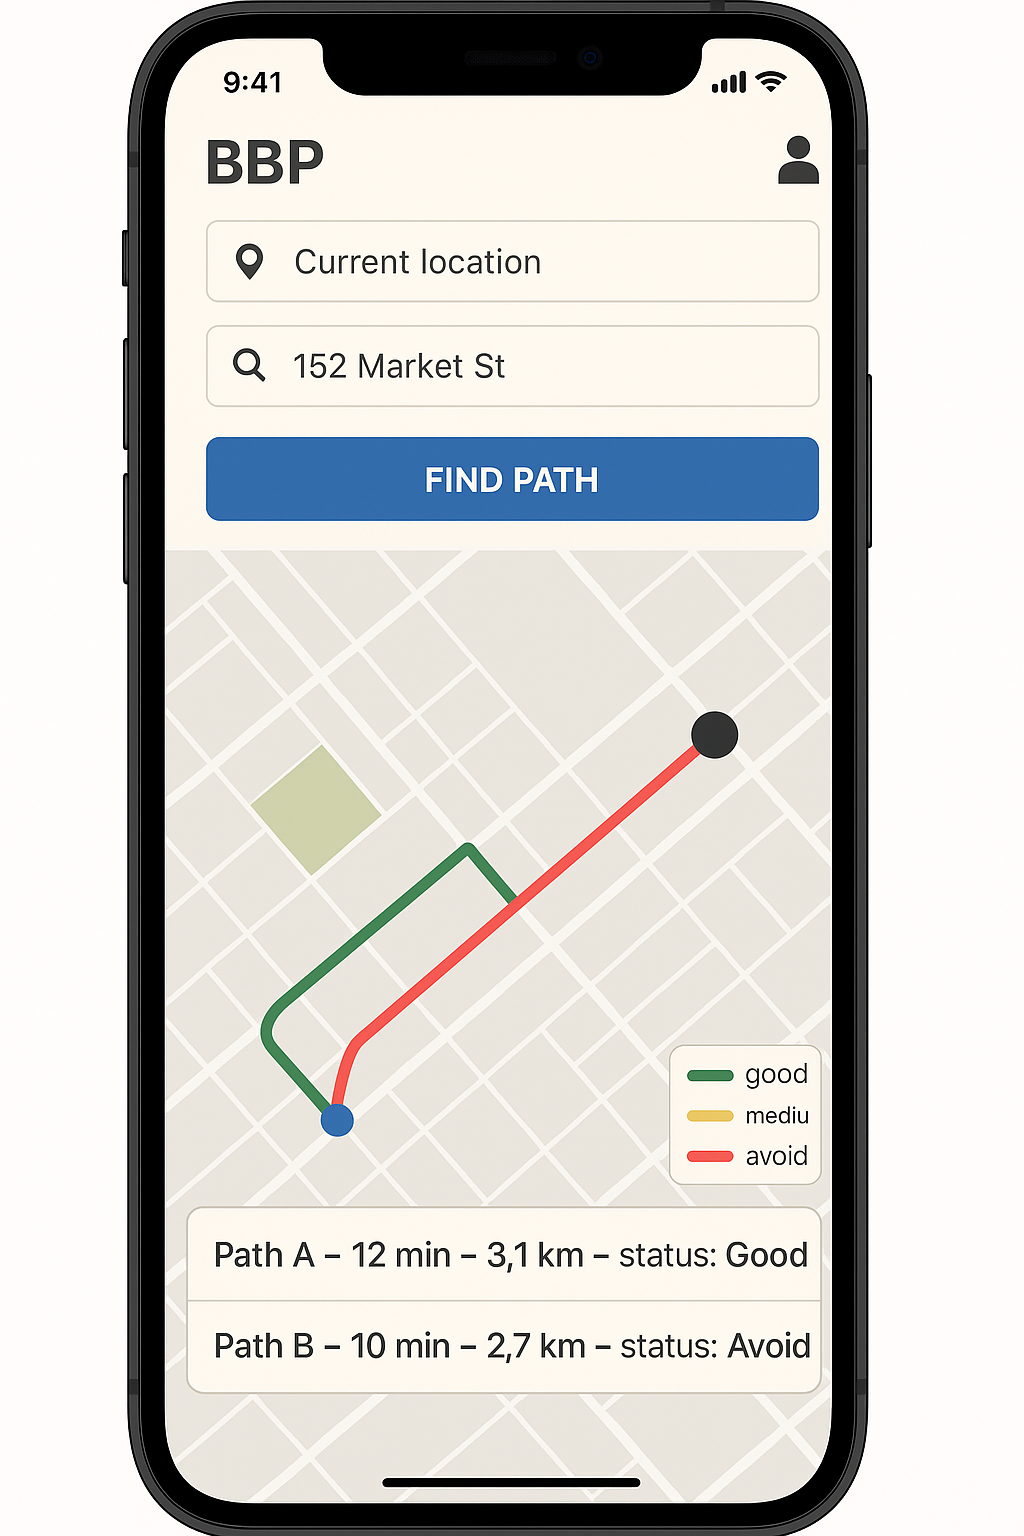
\includegraphics[width=0.4\textwidth]{Images/ui-home.png}
    \caption{Conceptual home / map screen for path search.}\label{fig:ui-home}
\end{figure}

The home screen (Figure~\ref{fig:ui-home}) is the main entry point for both unregistered users and
Bikers when searching for paths (F5). It corresponds to Scenario~S4 and to shared phenomena
SP6--SP7.

At the top, a simple form allows the user to specify an \emph{origin} and a \emph{destination}.
By default, the origin field is pre-filled with the current location, while the destination field
accepts a free-text address or point of interest. A prominent ``Find path'' button triggers the
path query.

The central area shows a map with the user position and the candidate paths between the chosen
origin and destination. At least two alternative paths are shown, using different colours to
represent their overall status (e.g., green for good, yellow for medium, red for avoid). A small
legend clarifies the meaning of these colours. A bottom sheet lists the candidate routes with
their main properties (estimated time, distance, summary status). Selecting a path in the list
highlights it on the map. This directly supports requirements RE-F5--1 to RE-F5--5.

\paragraph{Trip Recording screen}\mbox{}\\
\begin{figure}[H]
    \centering
    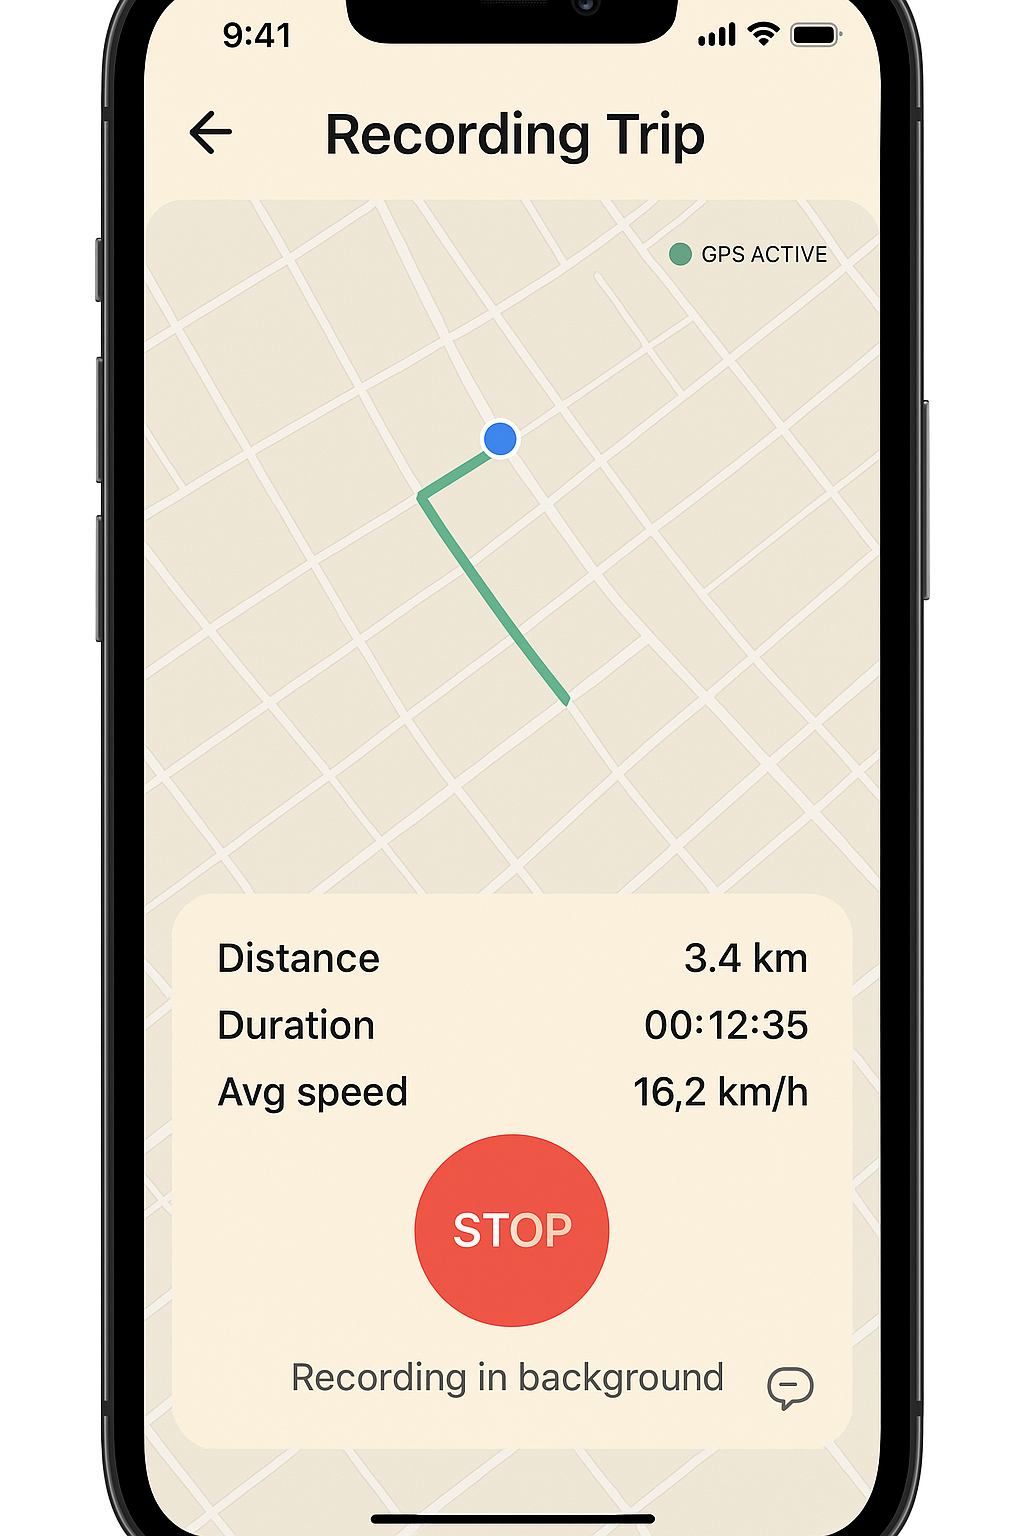
\includegraphics[width=0.4\textwidth]{Images/ui-recording.png}
    \caption{Conceptual trip-recording screen for registered users.}\label{fig:ui-recording}
\end{figure}
The trip recording screen (Figure~\ref{fig:ui-recording}) is available only to registered users
(Bikers). It supports Scenario~S1 and function F2.

The top bar indicates the current mode (e.g., ``Recording Trip''). The central map shows the
current GPS position and the portion of the path already travelled during the active trip. A small
indicator (e.g., ``GPS active'') provides feedback on sensor availability (SP2--SP3).

A stats panel above the bottom edge displays key trip statistics updated in real time:
distance, elapsed time, and average speed. A large, high-contrast button in the panel controls
recording: it appears as ``Start'' when no recording is active, and as ``Stop'' (or ``Pause'') while
recording is ongoing. A short status message (such as ``Recording in background'') confirms the
current state. An optional ``Add note / mark issue'' control lets the user drop a marker on the
current segment to be refined later in the contribution screen. Together, these elements support
requirements RE-F2--1 to RE-F2--6.

\paragraph{Manual Contribution / Path Information}\mbox{}\\
\begin{figure}[H]
    \centering
    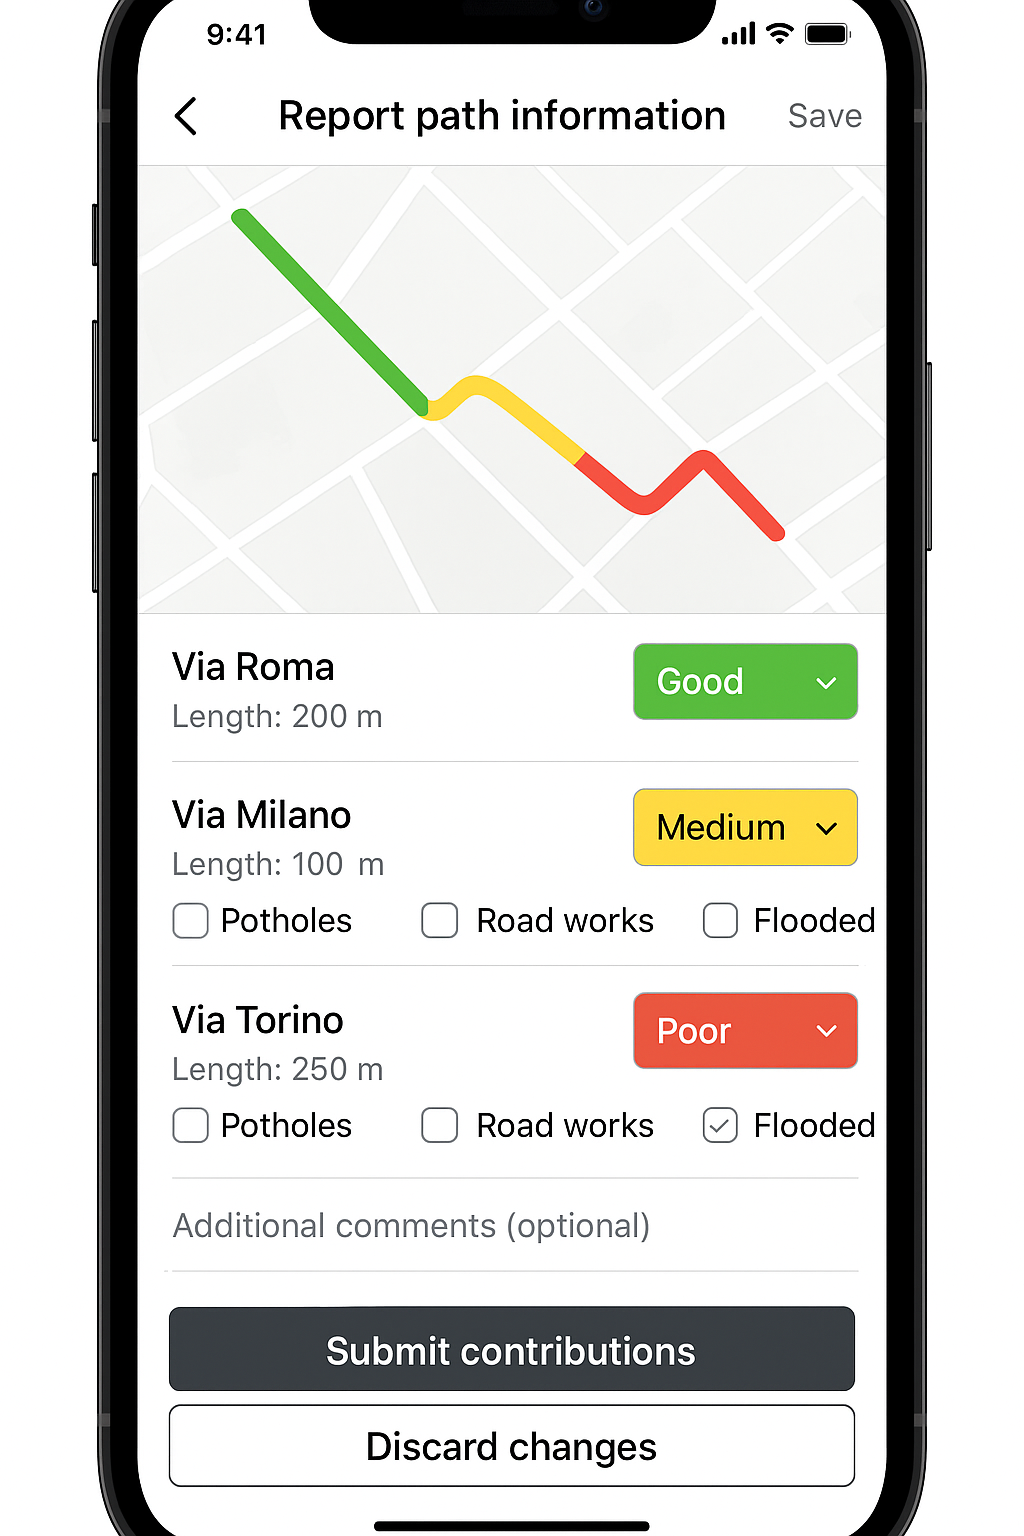
\includegraphics[width=0.4\textwidth]{Images/ui-manual.png}
    \caption{Conceptual manual contribution screen.}\label{fig:ui-manual}
\end{figure}
The manual contribution screen (Figure~\ref{fig:ui-manual}) is used by Bikers to insert and
update publishable information about the path segments they have travelled (Scenario~S2, function
F3, shared phenomenon SP4).

At the top, the map displays the most recently travelled path. The path is broken into separate
segments; each selected segment is shown in a colour that reflects its chosen status (e.g., green
for good, yellow for medium, red for poor/avoid). Below the map, a list contains one entry per
selected segment. Each entry shows:
\begin{itemize}
  \item the street name and approximate length;
  \item a drop-down menu to choose the segment status (Good / Medium / Poor / Avoid);
  \item checkboxes to indicate specific obstacles (e.g., potholes, road works, flooded);
  \item an optional text field for comments at the bottom of the list.
\end{itemize}
A primary ``Submit contributions'' button confirms the edits and stores them as publishable
information (RE-F3--2, RE-F3--4), while ``Discard changes'' allows the user to cancel the
operation without updating the stored data (RE-F3--3).

\paragraph{Validation of Automatically Detected Issues}\mbox{}\\
\begin{figure}[H]
    \centering
    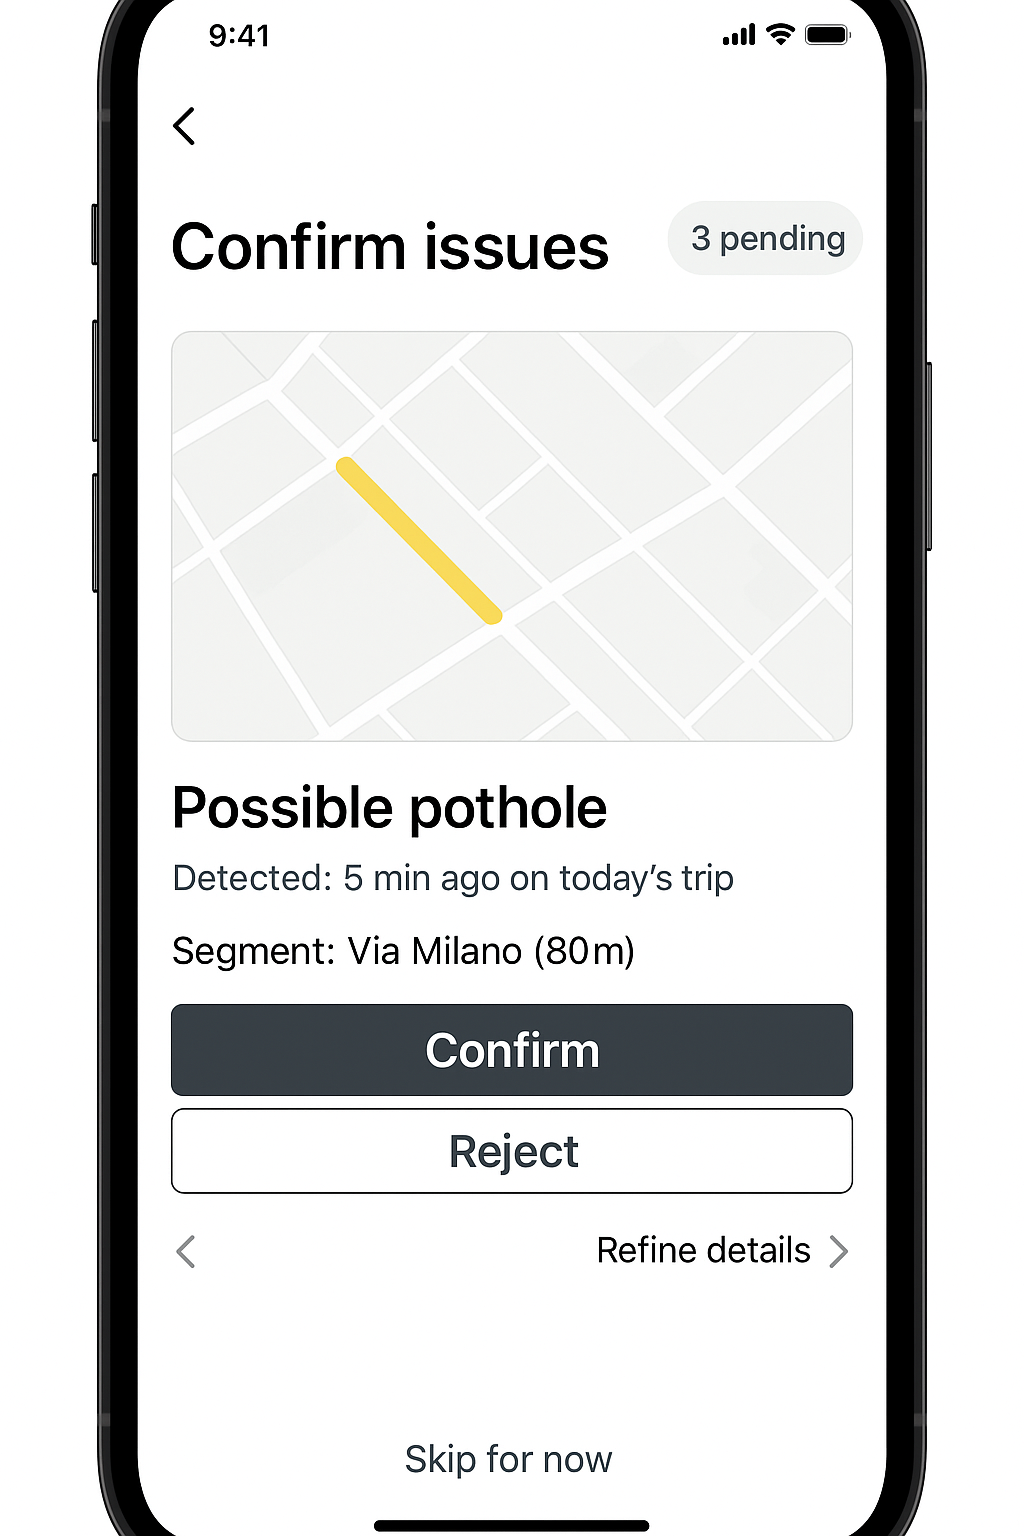
\includegraphics[width=0.4\textwidth]{Images/ui-confirm-issues.png}
    \caption{Conceptual screen for validating automatically detected issues.}\label{fig:ui-confirm-issues}
\end{figure}
The issue confirmation screen (Figure~\ref{fig:ui-confirm-issues}) is presented to Bikers when
BBP has inferred candidate Issues from sensor data collected during a recorded trip (Scenario~S3,
function F4, shared phenomenon SP5).

At the top, the screen shows the title (e.g., ``Confirm issues'') and the number of pending
candidate issues. The central panel displays one Issue at a time as a card containing:
\begin{itemize}
  \item a mini-map with the affected segment highlighted;
  \item a short textual description (issue type, detection time on the current trip, segment name
        and length).
\end{itemize}
Below the card, two large buttons allow the user to \emph{Confirm} or \emph{Reject} the candidate
Issue. A secondary text ``Refine details'' opens a compact form in case the biker wants to edit before confirming. A ``Skip for now'' action leaves the Issue in the
\textit{PendingValidation} state. Confirmed or refined Issues are stored as validated information,
while rejected Issues are discarded, in line with requirements RE-F4--2 to RE-F4--5.

\paragraph{Moderator Review screen}\mbox{}\\
\begin{figure}[H]
    \centering
    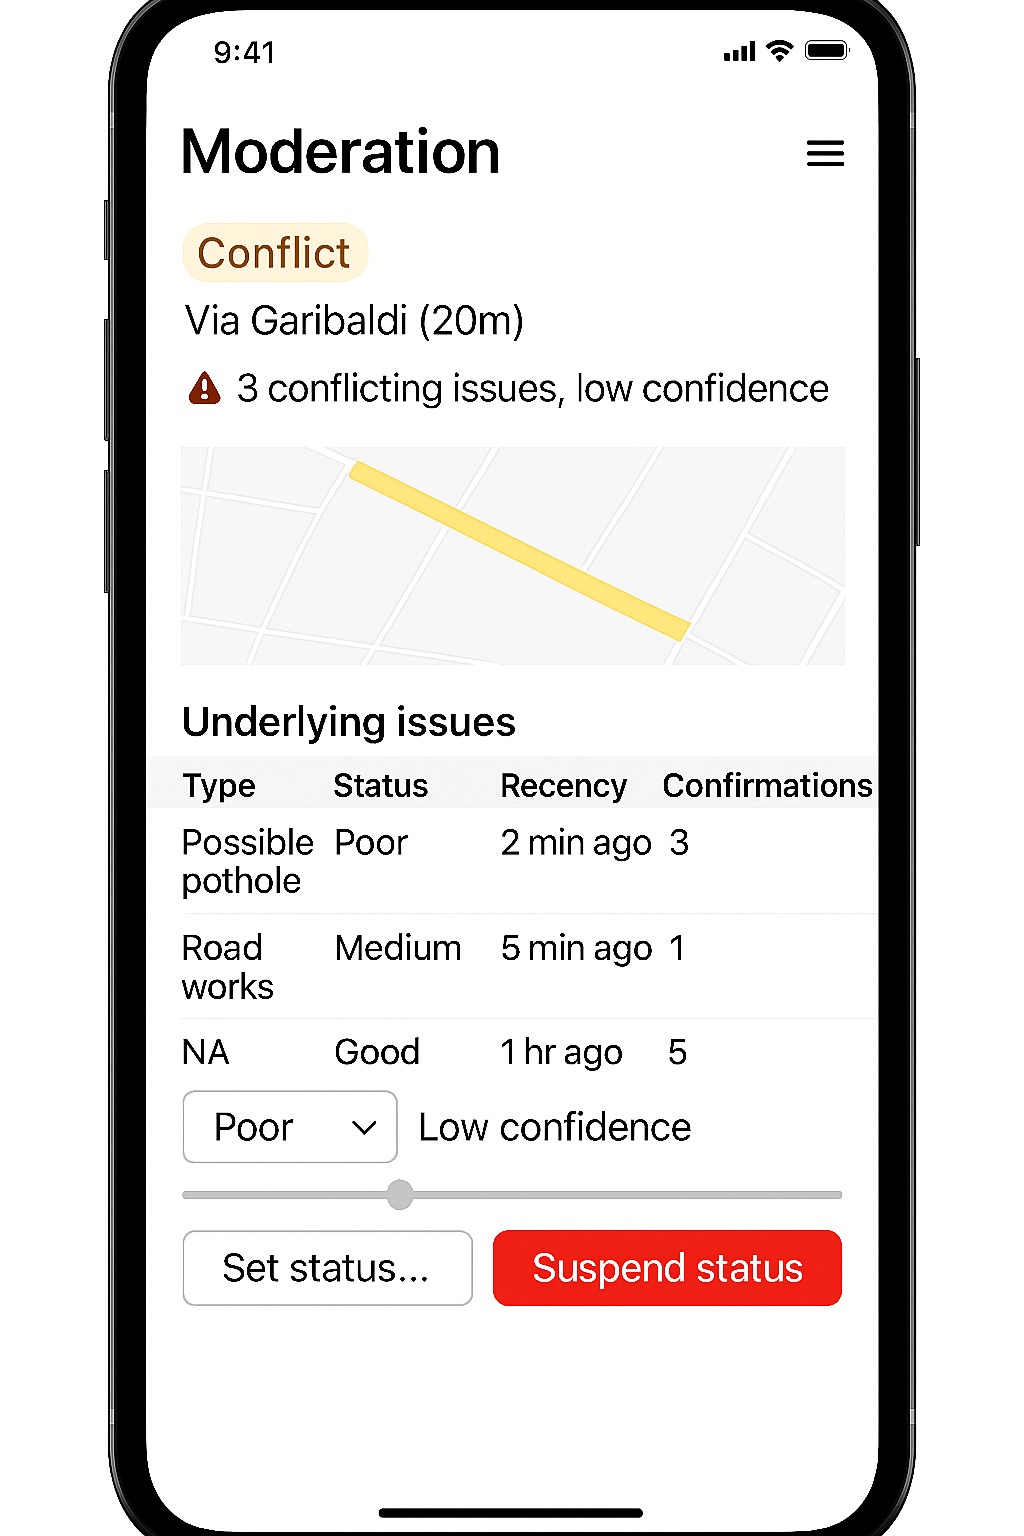
\includegraphics[width=0.4\textwidth]{Images/ui-moderation.png}
    \caption{Conceptual moderation screen for resolving conflicts.}\label{fig:ui-moderation}
\end{figure}
The moderation screen (Figure~\ref{fig:ui-moderation}) is intended for Moderators and supports the
conflict-resolution and aggregation behaviour described in Scenario~S5, function F6, and in the
SegmentStatus state diagram.

At the top, a summary shows the current problem segment (e.g., ``Via Garibaldi (20m)'') together
with a chip indicating whether its SegmentStatus is in \emph{Conflict} or \emph{Suspended}. A
short line summarises the situation (e.g., ``3 conflicting issues, low confidence''). Below, a map
highlights the affected segment.

The ``Underlying issues'' table lists the Issues that contributed to the conflict, with columns for
type, status (e.g., Good/Bad), recency (time since the report), and number of confirmations. This
directly addresses the aggregation and conflict-detection logic (F6).

At the bottom of the screen, some inputs allows the Moderator to:
\begin{itemize}
  \item choose a new published status for the segment from a drop-down menu (Good / Medium /
        Poor / Avoid);
  \item adjust a confidence value via a slider;
  \item apply the chosen status (``Set status'' button);
  \item temporarily hide the status by pressing a prominent ``Suspend status'' button, moving the
        SegmentStatus into the Suspended state.
\end{itemize}
These actions correspond to the transitions between \textit{Active}, \textit{Conflict detected},
\textit{Under moderation} and \textit{Suspended} in the SegmentStatus lifecycle.

\paragraph{Consistency with requirements}\mbox{}\\
The five screens described above collectively cover all the main interactions defined in the RASD:\
trip recording and review (G1, F2), manual contribution and maintenance of path information (G2,
F3), validation of automatically detected issues (G3, F4), path search and ranked presentation for
any user (G4, F5), and aggregation and moderation of contributions (G5--G6, F6).
They are intended as illustrative examples; the final implementation may vary in appearance as long
as these interaction patterns and information needs are preserved.

\subsubsection{Hardware interfaces}
BBP is designed primarily for smartphones carried by bikers and for server-side hardware operated by
the service provider.

\paragraph{Client devices.}

\begin{itemize}[noitemsep,topsep=0.4em]
  \item \textbf{Smartphone}: modern Android or iOS device.
  \item \textbf{Location and motion sensors}: integrated GPS receiver and inertial sensors inside the mobile,
        usually an accelerometer and a gyroscope. They help to measure position and motion data during trips.
  \item \textbf{Network connectivity}: Wi-Fi or mobile data (3G/4G/5G) to communicate with the BBP backend
        and external services.
\end{itemize}

The smartphone hardware is controlled by the user and its operating system. BBP can only access sensors
and networks that have been allowed by the users and their devices' OSes.

\paragraph{Server-side hardware.}

BBP backend services utilize general-purpose server hardware. No assumptions are made on the specific CPU,
memory, or storage configuration other than being sufficient to:
\begin{itemize}[noitemsep,topsep=0.4em]
  \item handle concurrent requests from client devices;
  \item store and retrieve trip records, path information, and user accounts;
  \item communicate with external map, traffic, and weather services.
\end{itemize}

Details of server provisioning and scaling are considered design and deployment concerns and are outside
the scope of this RASD.\

\subsubsection{Software interfaces}
BBP interacts with many external software systems, platforms and services.
\paragraph{Map / geocoding / routing service.}
An external map service provides:
\begin{itemize}[noitemsep,topsep=0.4em]
  \item digital map tiles for visualization in the client UI;\
  \item geocoding and reverse-geocoding of addresses and points of interest;
  \item routing between origin and destination, including alternative paths.
\end{itemize}
The interface is a web API invoked by the BBP backend; requests contain origin/destination coordinates or textual addresses, and responses contain route geometries, distances, and metadata.

\paragraph{Weather information service.}
A weather service provides current and recent weather conditions for given locations and times. BBP uses this interface to:
\begin{itemize}[noitemsep,topsep=0.4em]
  \item enrich trip records with observed weather conditions;
  \item optionally influence path ranking based on adverse weather.
\end{itemize}
The interface is a web API that accepts geographic coordinates and timestamps and returns structured weather data (e.g., temperature, precipitation, wind).

\paragraph{Mobile platform services.}
On client devices, BBP relies on operating system services exposed through standard SDKs:
\begin{itemize}[noitemsep,topsep=0.4em]
  \item location services (to access GPS position with user consent);
  \item sensor APIs (to read accelerometer and related motion data);
  \item network APIs (to perform secure HTTP requests to the BBP backend).
\end{itemize}
These interfaces are platform-dependent but are logically equivalent across supported mobile operating systems.



\subsection{Functional Requirements}\label{sec:functional_requirements}

This section defines the functional requirements of the Best Bike Paths (BBP) system.
Requirements are grouped according to the Product Functions F1--F6 defined in Section~\ref{sec:product_functions}.
Each requirement is labelled for traceability and later mapping to use cases.


\subsubsection*{F1 --- User Management}\label{sec:F1}

\begin{itemize}

    \item \textbf{RE-F1--1: Account Creation}\label{req:RE-F1-1}\\
    The system shall allow a person to create a registered user account, 
    provided they supply the information required for authentication.

    \item \textbf{RE-F1--2: User Authentication}\label{req:RE-F1-2}\\
    The system shall authenticate a user when valid credentials are provided.

    \item \textbf{RE-F1--3: Access Control}\label{req:RE-F1-3}\\
    The system shall restrict access to trip recording and contribution 
    functionalities to authenticated registered users only.

    \item \textbf{RE-F1--4: Unregistered User Access}\label{req:RE-F1-4}\\
    The system shall allow unregistered users to request bike paths and 
    view ranked results with no authentication.

    \item \textbf{RE-F1--5: Session Termination}\label{req:RE-F1-5}\\
    The system shall allow a registered user to log out, after which no 
    registered-only functionalities may be accessed.

\end{itemize}

% =========================================================
\subsubsection*{F2 --- Trip Recording and Review}\label{sec:F2}

\begin{itemize}

    \item \textbf{RE-F2--1: Start Trip Recording}\label{req:RE-F2-1}\\
    The system shall start recording a trip when a registered user initiates recording.

    \item \textbf{RE-F2--2: Stop Trip Recording}\label{req:RE-F2-2}\\
    The system shall stop trip recording when a registered user ends the trip.

    \item \textbf{RE-F2--3: GPS Data Acquisition}\label{req:RE-F2-3}\\
    The system shall acquire positional data (GPS coordinates) at regular intervals 
    during an active trip.

    \item \textbf{RE-F2--4: Sensor Data Acquisition}\label{req:RE-F2-4}\\
    The system shall acquire motion-related sensor data (accelerometer, gyroscope) 
    during an active trip.

    \item \textbf{RE-F2--5: Trip Statistics Computation}\label{req:RE-F2-5}\\
    The system shall compute trip statistics, including distance, duration and average speed, 
    after recording ends.

    \item \textbf{RE-F2--6: Weather Data Attachment}\label{req:RE-F2-6}\\
    The system shall retrieve and associate weather information with the recorded trip.

    \item \textbf{RE-F2--7: Trip History Presentation}\label{req:RE-F2-7}\\
    The system shall display a list of previously recorded trips for each registered user.

    \item \textbf{RE-F2--8: Trip Review}\label{req:RE-F2-8}\\
    The system shall display detailed information for any selected trip, including statistics 
    and associated weather information.

\end{itemize}

% ============================================================
\subsubsection*{F3 --- Manual Contribution and Maintenance of Path Information}\label{sec:F3}

\begin{itemize}

    \item \textbf{RE-F3--1: Manual Path Selection}\label{req:RE-F3-1}\\
    The system shall allow registered users to select travelled path segments for reporting.

    \item \textbf{RE-F3--2: Manual Issue Submission}\label{req:RE-F3-2}\\
    The system shall allow registered users to annotate selected path segments 
    with status or obstacle information.

    \item \textbf{RE-F3--3: Edit Existing Contributions}\label{req:RE-F3-3}\\
    The system shall allow registered users to update or remove their previously submitted 
    path information.

    \item \textbf{RE-F3--4: Publishable Information Storage}\label{req:RE-F3-4}\\
    The system shall store submitted or updated manual contributions as publishable 
    path information.

\end{itemize}

% ============================================================
\subsubsection*{F4 --- Automatic Detection and Validation of Issues}\label{sec:F4}

\begin{itemize}

    \item \textbf{RE-F4--1: Issue Inference}\label{req:RE-F4-1}\\
    The system shall infer candidate issues from motion-related sensor data collected 
    during a recorded trip.

    \item \textbf{RE-F4--2: Candidate Issue Presentation}\label{req:RE-F4-2}\\
    The system shall present inferred candidate issues to the user for validation 
    after the trip ends.

    \item \textbf{RE-F4--3: User Validation Actions}\label{req:RE-F4-3}\\
    The system shall allow users to confirm, reject or refine candidate issues.

    \item \textbf{RE-F4--4: Acceptance of Validated Issues}\label{req:RE-F4-4}\\
    The system shall store confirmed or refined issues as publishable information.

    \item \textbf{RE-F4--5: Discarding Rejected Issues}\label{req:RE-F4-5}\\
    The system shall discard rejected issues so that they do not influence 
    publishable path information.

\end{itemize}

% ============================================================
\subsubsection*{F5 --- Path Search and Ranked Presentation}\label{sec:F5}

\begin{itemize}

    \item \textbf{RE-F5--1: Path Query Input}\label{req:RE-F5-1}\\
    The system shall allow any user to provide an origin and a destination to request a bike path.

    \item \textbf{RE-F5--2: Path Computation}\label{req:RE-F5-2}\\
    The system shall compute one or more candidate paths between the specified origin 
    and destination, using external mapping or routing services when needed.

    \item \textbf{RE-F5--3: Path Ranking}\label{req:RE-F5-3}\\
    The system shall compute a path score for each candidate path using segment conditions, 
    quality indicators and path length.

    \item \textbf{RE-F5--4: Path Presentation}\label{req:RE-F5-4}\\
    The system shall present ranked paths and their associated properties to the user.

    \item \textbf{RE-F5--5: Path Details Display}\label{req:RE-F5-5}\\
    The system shall display detailed information for any selected path, including the 
    conditions of its constituent segments.

\end{itemize}

% ============================================================
\subsubsection*{F6 --- Aggregation and Maintenance of Path Knowledge}\label{sec:F6}

\begin{itemize}

    \item \textbf{RE-F6--1: Aggregation of Issues}\label{req:RE-F6-1}\\
    The system shall aggregate issues from multiple users for each path segment.

    \item \textbf{RE-F6--2: Freshness and Confirmation Priority}\label{req:RE-F6-2}\\
    The system shall resolve conflicts between issues by privileging fresher reports 
    and those with more confirmations.

    \item \textbf{RE-F6--3: SegmentStatus Update}\label{req:RE-F6-3}\\
    The system shall compute and update the SegmentStatus representing the current 
    publishable condition of each path segment.

    \item \textbf{RE-F6--4: Moderator Override}\label{req:RE-F6-4}\\
    The system shall allow moderators to override or correct aggregated segment statuses 
    when necessary.

    \item \textbf{RE-F6--5: Consistency of SegmentStatus}\label{req:RE-F6-5}\\
    The system shall ensure that at most one active SegmentStatus exists for each 
    path segment at any given time.

\end{itemize}
